% !TEX root = ../main.tex
\section{Setesh} \label{sec::setesh}
\DndDropCapLine{}{This city saved me when I was an}
\textit{orphaned child, sold into chains.
Now is my turn to save it.}

\hspace*{\fill} --- Kallias, Ophis Tower commander

Setesh is the favored polis of Karametra, and its buildings blend so perfectly into the forest that it's difficult to tell the difference between inside and outside.
The populace lives in harmony with the thick forests, terraced farms, and trained animals of Setesh, and they celebrate the cycle of seasons with grand holidays.

Setesh is also unique among the poleis of Viphoger in that few of its adult residents are gats.
Umans comprise the bulk of the population, holding almost all of the leadership roles and carrying out most work.
Gats are few and far between, and the other kins are even rarer in the polis.

The Seven Kingdoms of the Sea hold an intolerant attitude toward umans, where they are sold as slaves on most ports.
In Khedrat this situation is even more dire, where king Olag ordered the execution of all umans.
The ones that could escaped, and founded Setesh; hidden by the thick Nessian Wood.

% Children run freely around the polis.
% They're so important, in fact, that Setesh's people take in abandoned children from all over Viphoger.

\subsection*{People of Setesh}
    The populace of Setesh live in a beautiful paradise, and they're prepared to fight to the death to protect it.
    The constant training in archery, falconry, riding, and close combat can seem out of place among the idyllic forests and beautiful gardens and orchards, but that is the way of life in Setesh.

    \subsubsection{Gender in Setesh}
        Seteshans believe that women become heroes through martial exploits, while men do so by finding their own way in the world.
        As a result, the polis is populated mostly by women and children.

        When young men reach the age of fourteen, their rites of passage culminate in a journey called peregrination, where they wander the land until they find a new place to call home.
        The few men who reside permanently in Setesh live in the Amatrophon, training and caring for the animals there.
        Some of these men never peregrinated, but others left and then returned to Setesh.

        The women of the polis form a tight-knit community where property is held in common.
        There is no marriage, and ancestry is traced matrilineally.

        Despite the very different roles played by men and women, Seteshans are flexible when it comes to any individual's place in that structure.
        Some men set out on peregrination after spending a number of years identified as women, and some women return from peregrination (or never undertake it) after a period of realization.
        Some people move fluidly between roles, and a few choose a special role that Seteshans view as standing outside the dichotomy of gender, living in Ophis Tower.

        The warriors of Ophis Tower are martially trained as women are but wander the world as men do.
        They gather information for the Ruling Council, search out routes for peregrination (including identifying sympathetic individuals and households who will mentor young men at the start of their journeys), and rescue lost and abandoned children from other communities, bringing them back to Setesh.

    \subsubsection{The Ruling Council}
        Karametra is the queen of Setesh, but of course gods have more important concerns than the day-to-day governance of a uman polis.
        So a five-member council attends to the daily tasks of leadership on the deity's behalf.
        The council is made up of the commanders of the four prominent fortress-watchtowers that guard the polis.
        These commanders are elected by popular vote: Anthousa of Leina Tower, Phaedra of Hyrax Tower, Niketa of Bassara Tower, and Kallias of Ophis Tower.
        The fifth member is Silverbrow, a dratl ird oracle who reads the Kelema Veil at the Nexuses of the Seasons and advises action based on her visions.
        Anthousa is the head of the council, considered Karametra's closest advisor and the de facto ruler of the city.

    \subsubsection{Defenders and the Four Towers}
        Karametra includes defense of the home in her domains, and the residents of Setesh follow suit.
        Seteshan military forces are organized into four major regiments, each associated with a fortress tower.

        \subparagraph{Bassara Tower} The tower of the fox stands near the Summer Nexus and watches for interlopers who enter the Nessian Wood without permission.
        During their training, troops there focus on archery and guerrilla tactics.
        Their leader is Niketa, a woman in her fifties who spends most of her time in the tower since she parted ways with her partner.

        \subparagraph{Hyrax Tower} The tower of the falcon lies on the ridge near the Winter Nexus.
        Its regiment includes contingents of scouts and falconers.
        Its leader is Phaedra, a nineteen-year-old master falconer and orphan from Mephetis who was rescued by the Ophis regiment.

        \subparagraph{Leina Tower} The tower of the lion stands near Karametra's temple at the heart of Setesh.
        Its regiment, led by the hero Anthousa, is dedicated to the defense of the polis and the training of its children.
        The Leina warriors favor double-edged axes.

        \subparagraph{Ophis Tower} The tower of the serpent nestles at the center of Setesh.
        Its wandering warriors travel the world, working on behalf of the Ruling Council.
        Their leader is Kallias, who was sold into slavery as a child.
        They lost an eye and several fingers before they were rescued and brought to Setesh, where they have devoted themselves to saving others in a similar plight.

    \subsubsection{The ``Little Bears'' of Setesh}
        Children in Setesh are reared by the polis as a whole and treated with the highest respect; their welfare is paramount and their training is a significant part of every warrior's occupation.
        Orphans and abandoned children are sacred to Karametra, so they are brought into the city and tended just as Setesh's own children are.

        In contrast to the discipline associated with educating children in other poleis, Seteshan youngsters enjoy tremendous freedom.
        Called arkulli, meaning ``little bears'', they are welcome anywhere in the city.
        They often wander in and out of the temple, training grounds, the hall of the Ruling Council, the market, and anywhere else their paths take them.
        Such freedom is meant to cultivate a curious spirit and help the children find the path they're most interested in following later in life.

    \subsubsection{Nonumans in Setesh}
        Setesh doesn't welcome outsiders, as a rule, except the orphaned and abandoned children brought to live in the polis.
        But the polis can be more hospitable to nonuman outsiders than to umans (especially male umans) from other poleis.
        A few irds of the Vahagha band, leonin, and bughna gats have earned the right to live in Setesh.
        Dryads and naiads from the Nessian Wood rarely try to enter the polis, but they are often friendly with the Bassara soldiers who patrol the forest.

\subsection*{Features of Setesh}
    Setesh fuses nature and civilization into a single living organism.
    The polis extends from a huge tree at its center, like the rings of a still larger tree.
    A dense circle of vegetation forms the city's outer wall, with the treetops woven together to create a barrier against intruders.
    Expertly trained archers stand guard on platforms nestled among the upper branches.
    Inside these natural walls, patches of thick forest alternate with open spaces where the Seteshans build their homes and civic buildings amid the trees.
    Out of deference to Nylea, the residents of Setesh never construct a building that isn't absolutely necessary, and their homes and buildings are seamlessly integrated into the environment, with vegetation weaving together into walls or roofs.

    \subsubsection{Temple to Karametra}
        In the very center of the city is the temple to Karametra, patron of Setesh.
        Three ancient trees grow from an earthen rise and spiral around the heart of the city.
        The temple, built of glittering limestone, nestles amid the massive trunks.
        Strong magical wards protect the temple, since Karametra herself sits here when she visits her beloved polis.
        All manner of civic functions are based in the temple, and most of them are carried out by Karametra's attendants.
        These attendants serve as healers, advisors, teachers, chroniclers, and oracles.

    \subsubsection{Nexuses of the Seasons}
        Four holy sites, corresponding to the four seasons, stand in or near the polis and serve as temples --- primarily for the rites of Karametra and Nylea, but also to the other gods to an extent.
        These nexus points between the mortal world and Cosmos --- a phenomenon called the Kelema Veil --- are where omens manifest amid star fields that glitter in the shadows and where oracles seek messages from the divine. The four nexuses are each distinct in their own ways.

        \subparagraph{Spring Nexus} Associated with Karametra, the Spring Nexus is located in a lavish garden just behind her temple in the city of Setesh.
        A large arch of vines and flowers leads into the nexus itself and stays fresh and green all year long.
        Spring is the most celebratory time for Seteshans --- a time for planting and hope.
        Worshipers leave gifts for both Karametra and Nylea here.

        \subparagraph{Summer Nexus} Located in an olive grove west of the city proper, the Summer Nexus is covered by a leafy green canopy.
        As a shelter from summer's heat, the nexus is a favorite resting spot for people and animals alike, and Nylea and Iroas are worshiped here.

        \subparagraph{Autumn Nexus} Near the southern edge of Setesh, in an orchard filled with golden apples, a small cave behind a basalt arch holds a perpetually burning flame.
        Priests keep a strict rotation to ensure the fire never goes out, as it represents Purphoros's fire that keeps the world warm through the colder seasons and allows the autumn harvest.
        In addition to Purphoros, Seteshans come here to worship Iroas and Mogis, when necessary.

        \pagebreak

        \begin{tikzpicture}[remember picture,overlay]
            \node[anchor=north, yshift=0.10cm] at (current page.north) {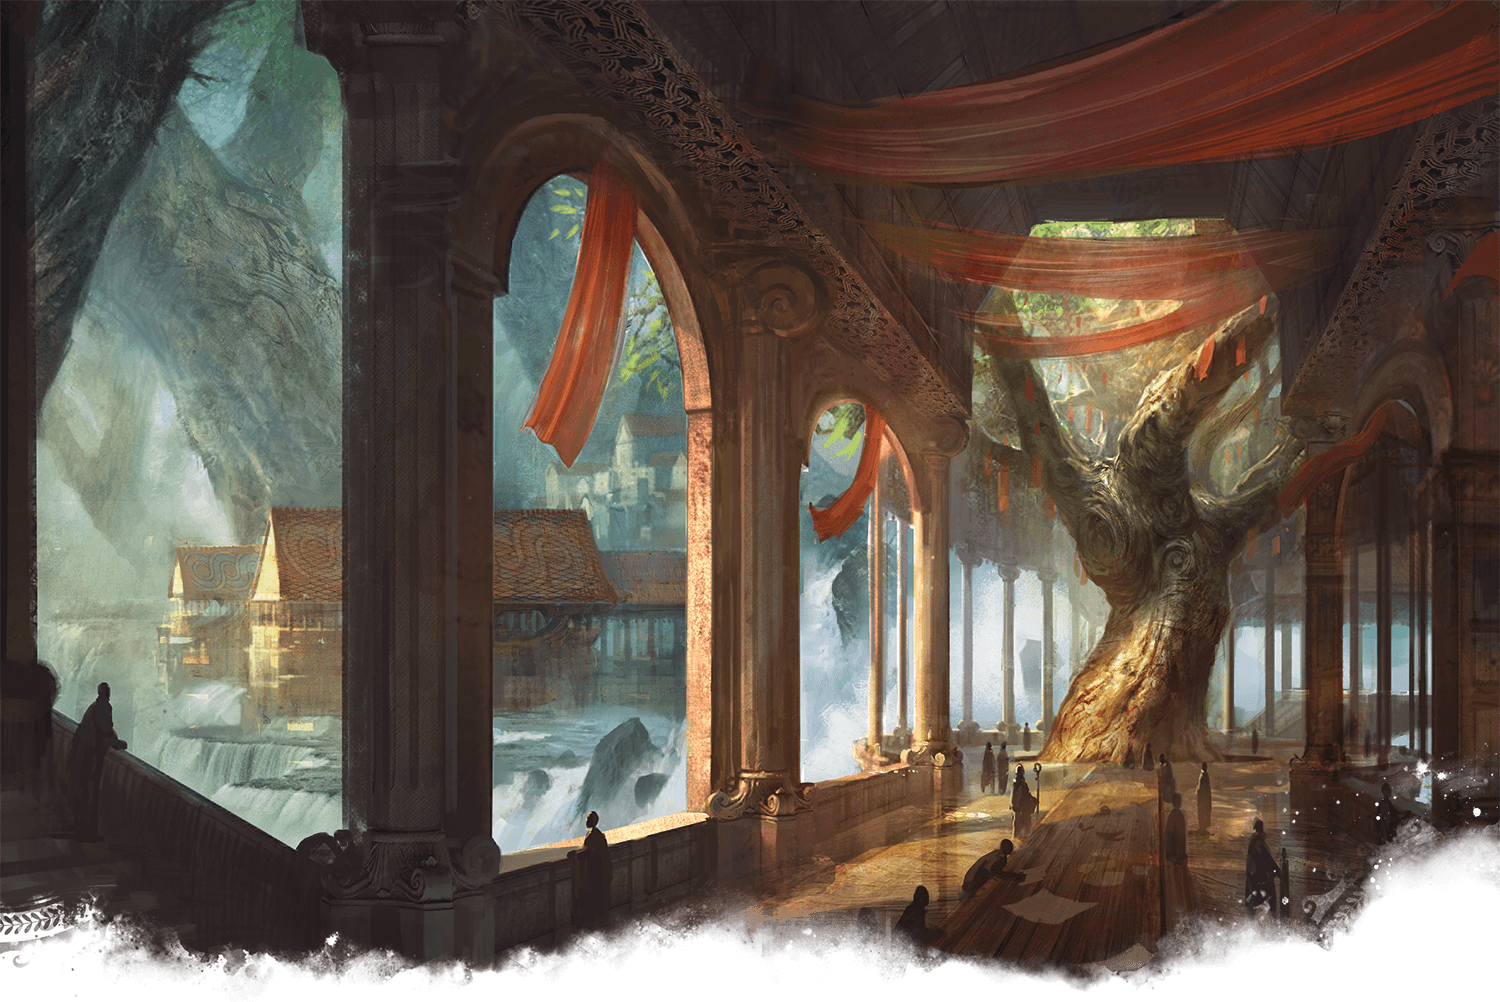
\includegraphics[width=\pdfpagewidth]{02viphoger/img/40setesh.png}};
        \end{tikzpicture}

        \vspace{12.5cm}

        \subparagraph{Winter Nexus} At the eastern edge of Setesh hides a rocky cave that was once a lion's den.
        The cave contains a burial ground and is rumored to lead all the way into the underworld.
        Seteshan children occasionally dare each other to see who can make it the farthest into the cave, but the morbid atmosphere usually sends the children scurrying back before long.
        Seteshans come here to worship Pharika and Erebos, paying respects to the dead or hoping to fend off death for a while yet.

    \subsubsection{Abora Market}
        The Abora Market is a giant, open-air market just inside the main eastern gate of Setesh.
        Every day it is thronged with citizens buying and selling food, crafts, and curiosities.
        On the seven days surrounding the full Fagal, outsiders are even allowed into the market, though they are still prohibited from roaming the rest of the polis.
        Visitors who try to explore beyond the market are typically banned from the polis and must forfeit any goods they brought into the city.

        The most impressive part of the market is the raptor hall, where falconers show off the trained raptors available for sale.
        Hunters all over the Viphoger come to buy famous Seteshan falcons.

        \pagebreak~
        \vspace{12.5cm}

    \subsubsection{Caryatid Groves}
        Scattered throughout the city are several groves that are sacred to Karametra and Nylea, made up of slender trees with almost umanlike forms.
        It is said that whoever enters one of these sacred groves in search of peace will find it --- and take root, becoming part of the grove.
        % NOTE: For the stats of the caryatids, use the Animated Tree.
        The trees here are caryatids, capable of animating in defense of the groves or the city but otherwise resting in silent stillness.

\subsection*{Setesh's Surroundings}
    Beyond the city's encircling trees, the territory of Setesh extends to cover about a third of the Nessian Wood and a wide swath of the open chaparral.
    In contrast to Mephetis and Akhosh, no villages or military outposts mark Seteshan territory, but a few key features in the Nessian Wood define the area under Seteshan control.

    \subsubsection{Amatrophon}
        The Amatrophon encompasses a large forested region at the southwestern edge of Seteshan territory, and it provides a safe haven and training ground for the diverse range of animals that occupy an honored place as natural protectors in Seteshan society.
        Experts train the renowned falcons of Setesh here, along with horses for riding and for combat.
        More unusual animals are found here as well: trainers work with boars, wolves, and lions to get them ready to accompany Seteshans in battle.
        Here men live and work alongside women, collectively training and caring for the animals that live here.

    \subsubsection{Nessian Wood}
        The vast wilderness of the Nessian Wood is considered Nylea's domain.
        Its trees are as old as the world, twining together to form an impenetrable canopy shielding the wood from Heliod's angry glare.
        Their roots stretch deep into the earth, and some say they drink from the Rivers That Ring the World, the waters of the Underworld.
        All manner of wild and strange creatures dwell in the Nessian Wood, far from the reach of civilization.

        Nylea allows limited hunting in the Nessian Wood, but she has been known to kill those who poach without her permission.
        Setesh's Bassara regiment helps the god keep an eye out for such illicit hunters, as well as any intruders who might bring danger upon the polis.

        \subparagraph{Cypress Gates} A natural gap between the Oranad Mountains and the Phoberos Canyon on the west side of the Milakul Swamp provides access into the Nessian Wood from the west.
        Ancient umans carved an impenetrable fortress into the mountains to guard the pass.
        Bassara patrols from Setesh still check in on the fortress regularly, and they occupy the fortress when there is reason to suspect danger from the west.
        More than once, though, patrols have reached the fort only to find something else has taken up residence, whether it be rowdy irds, grim Returned, or worse.

        \subparagraph{Hunter's Crossing} Setesh once extended its claim over more of the forests, establishing military outposts like those of Akhosh.
        At the western end of the woodlands, along the road from Kofos known as the Guardian Way, the ruins of a round tower lie beside a rushing stream.
        This marks the greatest extent of ancient Setesh's reach.
        A site of rich natural beauty, with lilacs growing along the riverbank and silver fish darting in startlingly clear water, it is abandoned by Setesh and favored by travelers as a resting point on the road before coming under the eaves of the forest.

\begin{DndComment}[float=h]{Myth of Nikaia the First Caryatid}
    A Seteshan archer named Nikaia claimed that she could outshoot anyone, even Nylea.
    Word of this unwise boast spread, and in response Nylea appeared at the next archery contest at the Spring Nexus.
    She challenged Nikaia to an impossible feat of archery: to shoot an arrow into one of the twin trunks of Kruphix's great tree at the edge of the world.
    Nikaia immediately realized that neither refusal, failure, nor success would forestall Nylea's wrath.
    Nonetheless, she held her head high, she and Nylea both let fly, and both arrows hit.
    Impressed by the mortal, Nylea took Nikaia to her sacred grove and planted her there as a caryatid, immobile but forever occupying a place of honor.

    Since then, Nylea has honored dozens of other champions and worthy mortals, blessing them with the long lives of mighty trees.
    The grown seedlings of Nikaia and Nylea's other favored continue to share their wisdom and protect Setesh to this day.
\end{DndComment}
